\chapter{Deep Networks}\label{ch_deepNets}
\chapterauthor{Jeff Yoshimi}

% Discuss deep fakes and GANs

The idea of re-mapping an input space to a hidden unit space in order to solve classification and regression problems is what drew neural networks out of its first ``dark age'' and back into the limelight, giving rise to an explosion of interest in engineering and connectionism in the 1980s and 1990s (chapter \extref{ch_history}). The internal representations of these networks--usually 3 layer networks trained by backprop--allowed them to solve previously unsolvable problems like XOR (figure \extref{xor_remapping}). These representations were often psychologically realistic (section \extref{internalRepsFF}). However, recall that a second  winter lay in wait, as machine learning models took over in the late 1990s and 2000s. What got us out of that second winter was \glossary{deep network}s, that is, networks with more than 3 node layers, trained using new tricks and techniques, like convolutional layers, the use of graphical processing units for fast parallel computation, and the Relu activation function discussed in chapter \extref{ch_act_functions}. These advances made it possible to use the same types network discussed in chapter \extref{ch_supervised_ff} on much more difficult problems.\footnote{This history is well told by Kurenkov in section 3 of \url{https://www.skynettoday.com/overviews/neural-net-history}. As he summarizes, ``Deep Learning = Lots of training data + Parallel Computation + Scalable, smart algorithms.''}  They also developed psychological and neurally realistic internal representations, and thus these networks are of considerable interest across the different domains of neural network research.
% Summarize main history in footnote. Vanishing gradients. Relu. Automatic differentiation. Availability of big data. GPU.
% Generalized techniques for effectively performing gradient descent on many kinds of architectures were developed. This is called automatic differentiation. Basically very complex calculus. These also made it possible to parallelize much of this work. A standardized language for discussing these networks also emerged, via the dominance of a few programs: keras, tensorflow, etc. 

In terms of engineering, these many-layered networks have been associated with huge improvements in image recognition, speech recognition, language translation, and in many other areas \cite{lecun2015deep, goodfellow2016deep}. They do this by creating hierarchies of representations, corresponding  to increasingly complex features of an input image. As we saw in chapter \extref{ch_neuro} (see figure \extref{deepLearning_Vision}) when such networks are trained to recognize images they develop internal representation that are extremely similar to those developed by the human visual  system. Thus they are relevant both to neuroscience (where they can describe the behavior of neurons in the visual system), and to psychology (where they can describe internal representations humans might rely on).
% More on engineering advances. The nature paper (lecun2015deep) has some helpful information at "first major application"

The topic of deep networks and deep learning are quite involved and the field is active and continues to grow (this is a preliminary chapter on the topic; it will be expanded in the future). Here we will describe some of the main concepts and some of their applications to neuroscience and psychology.

\section{Convolutional Layers}\label{convolutionalLayer}

% Mention that images are usually associated with several channels of information, hence the input image is really a tensor. Not sure where best to introduce that.
% Terminology: source layer, source image, pixel array

The key idea with a deep network is to use a special type of weight layer called a \glossary{convolutional layer} to efficiently learn to recognize features in a previous layer.\footnote{An outstanding visual discussion of the concept of a convolutions is at \url{https://youtu.be/KuXjwB4LzSA}} Until now we've been dealing with weight layers that connect all the nodes in a source layer to all the nodes in a weight layer; these are sometimes called ``dense layers'' or ``fully connected'' layers to contrast them with convolutional layers.\footnote{There are other types as weight layer as well, for example sparse layers.}  By contrast, convolutional layers involve a set of weights that are ``scanned'' or ``passed'' over the source layer's activations to produce activations in a target layer. Convolutions are so important to deep networks that the term ``convolutional neural network'' or ``CNN'' is sometimes used (on analogy with ANN for artificial neural network and RNN for recursive neural network, etc.)

To understand how a convolutional  layer works we can begin with the concept of a \glossary{filter} or \textbf{kernel}, which is the set of weights that is scanned over the source layer. The source layer of a convolutional layer is often itself a 2d array, prototypically an input image or a transformation of such an image, and so we can think of the source layer activations as pixels and the source layer as a pixel array (even when the input is not an image this language is useful). Filters are like pattern matchers that we slide across the pixel array, which ``light up'' most when they are on top of a similar patch. The filter is generally moved from left to right and top to bottom of the pixel array. At each stage of the scanning operation, it is multiplied by the patch of the pixel array it is on top of.\footnote{To get a better feel for how this works videos are  helpful. A good place  to start is with the first animated gif here: \url{https://stanford.edu/~shervine/teaching/cs-230/cheatsheet-convolutional-neural-networks} This video is also great: \url{https://youtu.be/KuXjwB4LzSA}.}  The multiplication is a dot product (see chapter \extref{ch_linear_algebra}),  where each weight in the filter is multiplied by the corresponding activation of the pixel array.  Recall that the dot product computes something like a similarity score: the more the filter and the pixels match,the greater the dot product will be. The resulting scalar is used to populate one activation in the target layer. Thus, the convolutional layer computes a kind of \emph{sliding dot product} with the source activations, which highlights where the filter matches the pixel array.\footnote{The number of pixels the filter moves at each step is called the \emph{stride}. One issue that comes up is the edges, which the filter can't be passed over. To handle this \emph{padding} can be added, in the form of extra zeros around the edges of the pixel array.}

The idea is illustrated in figures \ref{cnn_filter} and \ref{cnn_workedExample}. A $3 \times 3$ filter is passed over a source pixel array, from left to right and top to bottom. At each moment during this scanning process the dot product is computed between the filter and its ``receptive field'' in the source matrix (the part of the image the filter is on top of). The code used to generate figure \ref{cnn_workedExample} is available online, and can be used to play with these layers to get a feel for how they work.\footnote{See: \url{https://colab.research.google.com/drive/13kqHY0xs8VpLU6Sv7PYtgD6Ro7KdiqjY}.}

\begin{figure}[h]
\centering
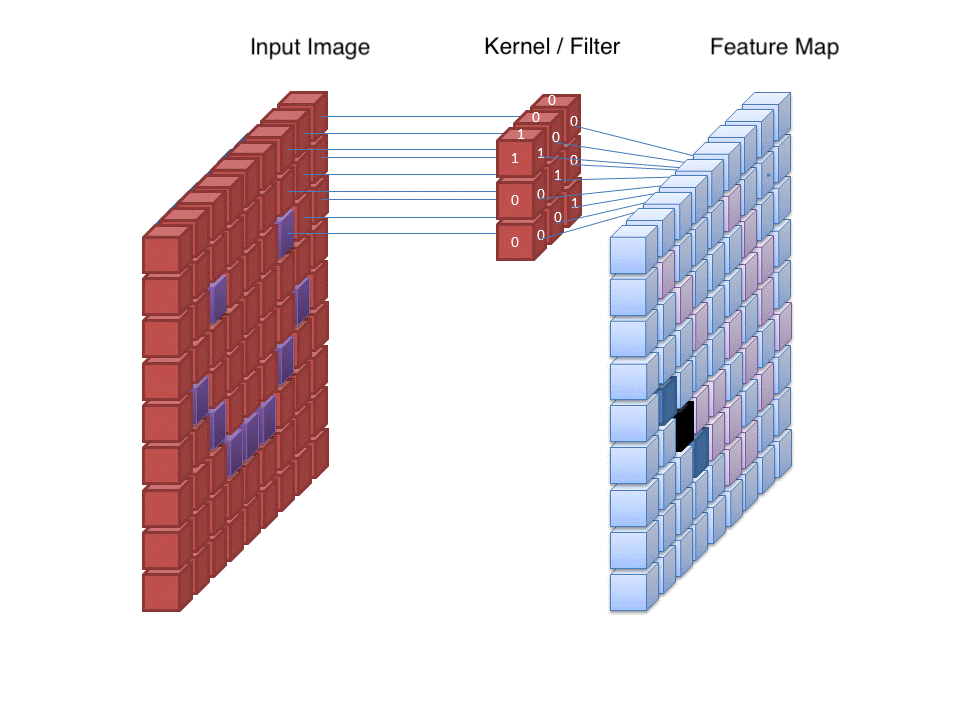
\includegraphics[width=0.5\textwidth]{images/CNN_Filter.png}
\caption[User Cecbur, \url{https://commons.wikimedia.org/wiki/File:Convolutional_Neural_Network_NeuralNetworkFilter.gif}, with labels added by Jeff Yoshimi.]{From left to right: an input image, a 3x3 convolutional filter (which detects edges with a $-45^\circ$ angle), and the resulting feature map. The filter is scanned across the image. At each stage of this scanning process, the dot product of the filtter's receptive field in the input image is computed and used to populate the feature map. This whole process is known as a convolution and a layer like this is a convolutional layer.}
\label{cnn_filter}
\end{figure}

% Link to colab notebook
In figure \ref{cnn_filter} the general idea is evident, but in figure \ref{cnn_workedExample} all the numbers are included so you can see how the computations are done. Since the input image and the filter are both binary, the dot product simply counts how many places the filter overlaps the image as it is scanned. In the example shown, it overlaps in one place, in the bottom right of the filter.  So that entry in the target layer is populated with a $1$.  Notice that this filter produces the highest value of $3$ only when it is directly on top of the line in the source layer. Try to understand how all the target layer activations are computed. You can also imagine what would happen if the filter or the image were changed.

\begin{figure}[h]
\centering
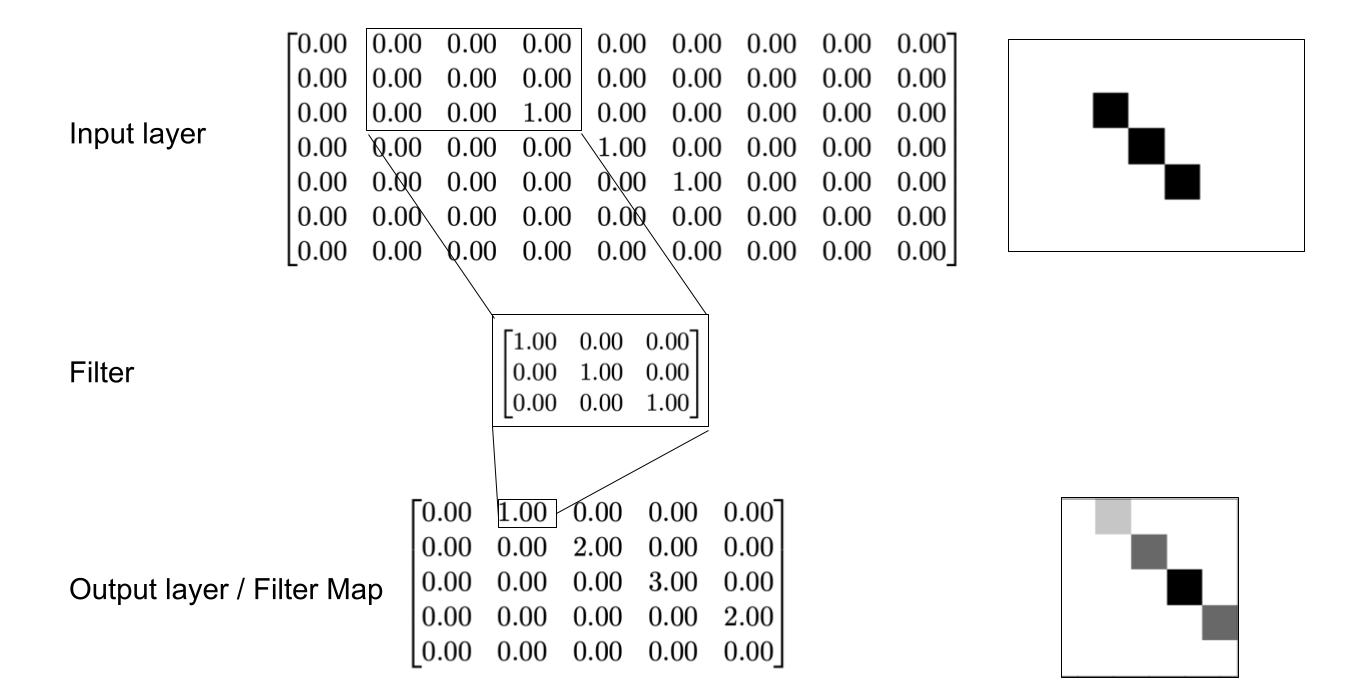
\includegraphics[width=0.8\textwidth]{images/CNN_WorkedExample.png}
\caption[Jeff Yoshimi]{Worked example of a convolutional layer. Notice that the feature map has the highest values where the filter matches the pixel array. In the case shown, the filter matches the pixel array in one pixel only. Imagine the filter sliding over the pixel array, and computing dot products (here: numbers of matching $1$'s), which are used to populate the feature map.}
\label{cnn_workedExample}
\end{figure}

The output or target layer of a convolutional layer is called a \glossary{feature map}. In these examples, the filter is an edge detector, that detects edges at a $-45^\circ$ angle, that is, edges shaped like a backslash `\textbackslash'. In the resulting feature map, notice that the activation is highest when the filter is directly on top of such an edge. In figure \ref{cnn_workedExample} the output layer / feature map activations simply correspond to how many pixels the filter and image overlap on: as you can see, the values are $1$, $2$, or $3$, and it is higher, the more edge like a given patch is. Thus, the feature map shows where this kind of edge occurs in the input image. It itself a new node layer, a new pixel array, a ``convolution'' of the previous one, that emphasizes the edges in the input image.

Again, note that this is totally different from the weights we have been studying throughout the book: there are no fixed connections at all. Instead it is like there is a little floating scanner that gets passed over source layer activations to produce output activations.

Also note that this edge detector is not programmed in. This is a neural network after all, and neural networks are trained, not programmed (section \extref{intro_comp_nn}), usually using a form of gradient descent (section \extref{sect_gradient_descent}). There is a performance advantage to these convolutional layers. All that must be trained is (in the example shown in figure \ref{cnn_filter}) $3 \times 3=9$ weights, rather than the $100 \times 100 = 10,000$ weights that would be required in a fully connected dense layer from the input layer to the feature map. This is a huge performance gain and part of what  made it possible with deep learning to train such large networks.

\section{Feature Maps and Tensors}

The magic really starts to happen when we train a \emph{set of filters}, each of which produces a separate feature map.  Figure \ref{deep_net2} illustrates the idea. Note how several of the node layers say ``Feature maps'' plural, or ``F.maps.'' Each feature map in one of these sets is a response to a different filter, for example, edges of different orientation. This is exactly how primary visual cortex reacts to images, so this is a nice model of the brain, hence an example of computational  neuroscience. However, these networks are best known for the engineering benefits, since they are powerful pattern recognition systems.


\begin{figure}[h]
\centering
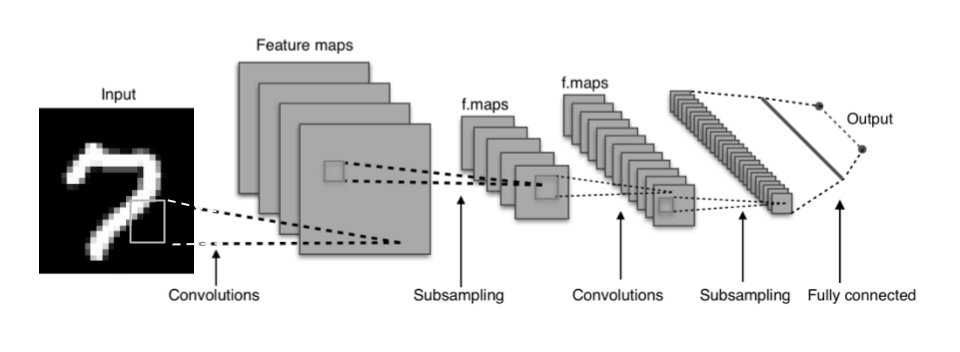
\includegraphics[scale=.45]{./images/deepNet.png}
\caption[Adapted from a creative commons image by Aphex34 at \url{https://commons.wikimedia.org/wiki/File:Typical_cnn.png} ]{A deep neural network, trained to recognize images. The convolutional layers scan over the inputs they are linked to. }
\label{deep_net2}
\end{figure}

A few things to note here.

First, a set of feature maps can be thought of as corresponding to a new kind of node layer. It is not just a  single set of nodes, but rather is itself a whole array of matrices. It's like a stack of pancakes, if each pancake is a matrix.  An array of matrices is a special kind of \glossary{tensor} (a generalization of the vectors and matrices we discussed in chapter \extref{ch_linear_algebra} to more complex numerical structures), and so computations in deep networks often involve the use of tensor mathematics.\footnote{Technically numbers and vectors and matrices are also tensors. The rank of a  tensor is the number of indices it takes to specify an ``entry'' in the tensor. A number is rank 0 because it requires no indices. Recall that a vector is like a list of numbers. A vector is rank 1 because it takes one index to specify an entry in a vector. A matrix is rank 2 because it takes two numbers to specify an entry (a row and column). A set of matrices is rank 3, because it takes 3 indices to specify an entry: one to specify a location in the array, and then a row and column index.}  
% Redundant with data science discussion

Second, these networks developing meaningful representations with training; the representations are not programmed in. This is kind of remarkable to ponder. We did not tell the network we want it to learn to respond to edges. All we focus on in training a network is inputs and outputs, using a labeled data set.  In the case shown in the figure, the training data involve images paired with numbers. The network is given nothing else but these training examples: if you see this picture, it's a 2; this picture is an 8, etc. Then the network adjusts all its parameters (all the weights in its convolutional layers), in such a way as to reduce error.  Edge detectors were learned by training, not programmed in. This is an old connectionist theme. In Nettalk (section \extref{internalRepsFF}), phonetic categories like consonant and vowel were not programmed in, but emerged with training. With simple recurrent networks  (section \extref{internalRepsRecurrent}), grammatical categories like verb and noun were not programmed in but  emerged with training.

\section{The many layers of a deep network}

In a full deep network many convolutional layers and regular ``dense'' weight layers are combined, sometimes as many as 100 or more! This allows the network to learn to identify not just simple features like edges or curves, but also \emph{features of features}, like combinations of curves which make more complex shapes, and then combinations of these shapes. 

% Improve discussion of location invariance
As can be seen in figure \ref{deep_net2}, there are other kinds of layers besides convolutional layers. Subsampling refers to methods where the size of a representation is reduced, often by scanning over the source layer, and then averaging or finding the largest value in each window (\emph{average pooling}, \emph{max pooling}, etc.).  This is also called downsampling.  
% More on value of downsampling / subsampling
% Mention flattening, which is just a shape change required to link the ``pixel array'' layers (matrices in rank 3 tensors) to a classical backprop style network.

The final layers of a deep network are often more conventional fully-connected dense layers. The idea is to start with layers that learn these complex features, then to compress these representations with subsampling, and finally to present the results to the final layers, which are basically familiar backprop networks presented with the results of a whole lot of convolving and subsampling.

\section{Applications of Deep Learning}

% This section obviously needs to be developed
% What do convolutional layers correspond to in the brain?
 
As discussed in section \extref{deep_revolution}, deep networks and deep learning led to a revolution in neural networks beginning in the 2010s. The revolution was in engineering initially, but the history of deep networks shows that they have applications across all the domains of neural network research: engineering, computational neuroscience, connectionism, and computational cognitive neuroscience. 

Deep network models originate in  computational neuroscience models of vision that were developed in the 1970s and 1980s \cite{fukushima1982neocognitron}.  These ideas were later used to engineer pattern recognition networks. A famous early application was recognizing zip codes written on envelopes \cite{lecun1989backpropagation}. As deep networks became mainstream based on technical improvements (big data, GPU and hardware acceleration, better architectures and training algorithms), scientists began using them, for example, to model the response profile of neurons in the visual system (recall the discussion of figure \extref{deepLearning_Vision} in chapter \extref{ch_neuro}). 

The idea is also relevant to connectionism and computational cognitive neuroscience. You may recall from the history chapter that concept of layered feature detection goes  back to Oliver Selfridge and his ``pandemonium'' model, which at the time just speculated that in seeing letters a hierarchy of ``demons'' pass messages along: from edge demons to curve edges and finally to the output layer's ``B demon'' (see figure \extref{selfridge} in chapter \extref{ch_history}). Deep networks instantiate this idea, in such a way that we can actually  see what their receptive fields are.\footnote{The receptive fields can be quite strange and even disturbing. See \url{https://distill.pub/2017/feature-visualization/} for some striking demonstrations.}  The significance of these networks for psychology is still in its infancy, but early results are promising \cite{zorzi2013modeling, ritter2017cognitive}.
% Work more on interpreting what is happening in that distll article, and add some material here, including pictures of the weird features. Then add some colab demos to the course.
